% =====================================================================
%  capitulos/06_anexos.tex  --  Anexos (A, B, C, ...)
%  Va después de \appendix en main.tex (que los numera A, B, ...); el rótulo
%  "Anexo" lo fija \renewcommand{\appendixname}{Anexo} en main.tex.
% =====================================================================

\chapter{Manual de instalación}
\label{anexo:instalacion}

EduFEM se distribuye por dos vías: un instalador para Windows —la vía recomendada para el estudiante—, que despliega el software como paquete autocontenido, y la instalación desde el código fuente para su inspección o extensión. El código está disponible en el repositorio público del proyecto\footnote{\url{https://github.com/Sucullani/SoftwareED}}.

\section{Instalación en Windows}

EduFEM se distribuye como un instalador único (\texttt{EduFEM-Setup.exe}) que copia el software, crea accesos directos en el menú Inicio y en el escritorio —identificados por el icono de la herramienta (\autoref{fig:logo-edufem})—, asocia la extensión \texttt{.edufem} de los proyectos para que se abran con doble clic y registra un desinstalador. La instalación se realiza por usuario, sin privilegios de administrador. Requisito: Windows 10 u 11 de 64 bits.

El paquete es autosuficiente en un sentido estricto: el empaquetado con \texttt{PyInstaller} incorpora el intérprete de Python y todas las bibliotecas, y el instalador añade la distribución \LaTeX{} reducida que describe la \autoref{sec:stack}, instalada junto al ejecutable. En consecuencia, el equipo de destino no necesita Python, ni una distribución \LaTeX{} previa, ni conexión a internet durante la instalación o el uso. Esta decisión responde a una dificultad observada en la práctica: cuando la memoria de cálculo se compilaba con la distribución \LaTeX{} que hubiera en el equipo, una instalación mínima interrumpía la exportación con un cuadro de diálogo por cada paquete ausente. Si falta la carpeta con el motor \LaTeX{}, el software recurre a la distribución que encuentre instalada en el sistema y, en su defecto, informa el problema; las fórmulas que se muestran en pantalla no dependen de \LaTeX{} en ningún caso.

Una restricción heredada de \TeX{} Live condiciona la carpeta de instalación: su motor no resuelve rutas que contengan tildes o espacios. Como el destino habitual de una instalación por usuario incluye el nombre del perfil de Windows, el asistente comprueba si esa ruta contiene tildes o espacios y, en ese caso, propone instalar en \texttt{C:\textbackslash ProgramData\textbackslash EduFEM}, que un usuario sin privilegios puede crear igualmente.

Al no estar firmado con un certificado comercial, la primera ejecución del instalador puede mostrar el aviso de Microsoft Defender SmartScreen (\enquote{Windows protegió su PC}), habitual en aplicaciones nuevas; se continúa con \emph{Más información} y \emph{Ejecutar de todas formas}. Una vez instalado, EduFEM se abre desde su icono como cualquier otra aplicación, sin nuevos avisos.

\section{Instalación desde el código fuente}

Para docentes o desarrolladores que deseen inspeccionar o modificar el software:

\begin{enumerate}
    \item Instalar \textbf{Python 3.11 o superior} (el desarrollo se realizó con la versión 3.13).
    \item Clonar el repositorio y ubicarse en su carpeta:
\begin{verbatim}
git clone https://github.com/Sucullani/SoftwareED.git
cd SoftwareED
\end{verbatim}
    \item Crear y activar un entorno virtual (recomendado):
\begin{verbatim}
python -m venv .venv
.venv\Scripts\activate
\end{verbatim}
    \item Instalar las dependencias:
\begin{verbatim}
pip install -r requirements.txt
\end{verbatim}
    \item Ejecutar EduFEM:
\begin{verbatim}
python main.py
\end{verbatim}
\end{enumerate}

\section{Dependencias}

El núcleo numérico y la interfaz se apoyan en bibliotecas de código abierto: NumPy y SciPy (cálculo), \texttt{ttkbootstrap} (interfaz), \texttt{pylatex} (memoria de cálculo y documentos de teoría), \texttt{Pillow} (figuras) y \texttt{ezdxf} (importación DXF). A ellas se añaden \texttt{matplotlib}, para los gráficos de los módulos educativos, la vista 3D y el círculo de Mohr, y \texttt{sympy}, para las expresiones simbólicas de los módulos y de la memoria de cálculo. A ellas se suma un componente externo al ecosistema de Python: el motor \texttt{pdflatex} que compila la memoria de cálculo, provisto por la distribución \LaTeX{} reducida que acompaña al instalador. Quien trabaje desde el código fuente puede generar esa distribución con el guion incluido en el repositorio o bien apoyarse en una instalación de \LaTeX{} propia. El motor numérico está vectorizado por lotes en NumPy puro ---calcula todos los elementos a la vez con operaciones sobre arreglos, en lugar de recorrerlos uno por uno---; así, las mediciones de tiempo del \autoref{cap:resultados} se reproducen con las dependencias listadas, sin compiladores ni aceleradores adicionales.


\chapter{Manual de uso}
\label{anexo:manual}

Este anexo describe el trabajo con EduFEM, desde la construcción del modelo hasta la interpretación de los resultados. El diseño de cada componente y su justificación están en la \autoref{sec:diseno-edufem}; aquí se indica cómo operarlo. El software organiza ese trabajo en tres fases ---pre-proceso, proceso y post-proceso--- accesibles mediante pestañas, que comparten un único lienzo central, es decir, el área gráfica donde se dibuja el modelo. La barra de menús se reduce deliberadamente a tres entradas: \textsf{Archivo}, \textsf{Modelo} y \textsf{Ayuda}.

La \autoref{fig:app-completa} muestra la ventana principal en la fase de pre-proceso, con sus tres zonas: el cuaderno de tablas, el lienzo compartido y la barra de estado.

\begin{figure}[htbp]
\centering

\includegraphics[width=\linewidth]{fig_app_completa}
\caption[Ventana principal de EduFEM en la fase de pre-proceso.]{Ventana principal de EduFEM en la fase de pre-proceso. A la izquierda, el cuaderno de tablas editables (con la tabla de \textsf{Nodos} activa); a la derecha, el lienzo compartido con el modelo del ejemplo canónico ---nodos, elementos, la carga nodal, los apoyos y los ejes---. La barra de estado inferior resume el diagnóstico de salud, el tipo de análisis y el recuento de grados de libertad.}
\label{fig:app-completa}
\end{figure}

\section{Pre-proceso: construcción del modelo}

La fase de pre-proceso (identidad cromática azul) reúne la definición geométrica y de cargas. A la izquierda, un cuaderno de cinco tablas editables ---\textsf{Nodos}, \textsf{Elementos}, \textsf{Cargas}, \textsf{Restricciones} y \textsf{Carg.\ Superf.}--- permite la entrada y edición directa de cada entidad; a la derecha, el lienzo refleja el modelo en tiempo real.

\subsection{Definición de la geometría}

Existen tres vías para construir la malla:

\begin{itemize}
  \item \textbf{Edición en tablas.} El doble clic en una celda abre el editor, y el doble clic en la fila atenuada del pie de cada tabla (\emph{placeholder}, es decir, la fila que reserva el lugar del registro siguiente) crea un registro nuevo con valores por defecto, que luego se completa. Se admite el pegado de bloques de texto tabulado desde una hoja de cálculo (Ctrl+V) para el alta masiva.
  \item \textbf{Modo dibujo (tecla D).} Al estilo de un programa de dibujo asistido, el usuario marca cuatro vértices sobre el lienzo ---con anclaje automático a los nodos existentes--- y el elemento cuadrilátero se crea al cuarto clic, corrigiendo de oficio la orientación antihoraria.
  \item \textbf{Importación.} Desde \textsf{Archivo} $\rightarrow$ \textsf{Importar} se carga geometría en formato DXF (polilíneas cerradas de cuatro vértices en la capa \texttt{FEM\_ELEMENTS}) o las entidades de un modelo en CSV/Excel.
\end{itemize}

\subsection{Propiedades del modelo}

El menú \textsf{Modelo} agrupa, en el orden lógico de definición de un problema de elementos finitos, cinco diálogos: \textsf{Tipo de Elemento} (Q4 o Q9), \textsf{Unidades} (ocho sistemas predefinidos con conversión automática de los valores), \textsf{Materiales} (módulo de elasticidad $E$, coeficiente de Poisson $\nu$ y densidad $\rho$), \textsf{Gravedad} (vector de aceleración y su activación) y \textsf{Tipo de Análisis} (tensión o deformación plana). Al cambiar de Q4 a Q9, los cinco nodos adicionales por elemento ---cuatro de arista y el central--- se generan automáticamente. La \autoref{fig:dialogo-material} muestra, a modo de ejemplo, el diálogo de materiales.

\begin{figure}[htbp]
\centering

\includegraphics[width=0.72\linewidth]{fig_dialogo_material}
\caption[Diálogo de materiales.]{Diálogo \textsf{Modelo} $\rightarrow$ \textsf{Materiales}: la lista de materiales definidos a la izquierda y el formulario de propiedades ($E$, $\nu$, $\rho$) a la derecha.}
\label{fig:dialogo-material}
\end{figure}

El diálogo \textsf{Tipo de Análisis} (\autoref{fig:dialogo-analisis}) ilustra con animaciones la distinción entre tensión plana ($\sigma_z = 0$) y deformación plana ($\varepsilon_z = 0$), las dos hipótesis bidimensionales que el software resuelve.

\begin{figure}[htbp]
\centering

\includegraphics[width=0.72\linewidth]{fig_dialogo_analisis}
\caption[Diálogo del tipo de análisis.]{Diálogo \textsf{Modelo} $\rightarrow$ \textsf{Tipo de Análisis}: la selección entre tensión plana (placa delgada cargada en su plano, $\sigma_z = 0$) y deformación plana (sólido largo confinado, $\varepsilon_z = 0$), con una animación ilustrativa de cada hipótesis.}
\label{fig:dialogo-analisis}
\end{figure}

\subsection{Cargas y restricciones}

Las cargas nodales, las cargas de superficie (carga distribuida sobre una arista, con su ángulo de aplicación) y las restricciones (empotramiento, rodillo en $x$ o en $y$) se definen en sus tablas respectivas o seleccionando la entidad en el lienzo, que pre-rellena una fila «fantasma» con valores por defecto. Los símbolos siguen la convención estructural habitual: triángulo con achurado para el empotramiento y triángulo sobre rodillo para los apoyos deslizantes.

\section{Proceso: resolución y exploración didáctica}

La fase de proceso (identidad cromática naranja) alberga los módulos educativos. La tecla F5, o el cambio a la pestaña de post-proceso, dispara la resolución, que antes revisa el modelo con un comprobador de salud (\autoref{fig:validador-salud}). Un error crítico detiene la resolución y se reporta con sugerencias de corrección; el usuario solo puede continuar si elige \textsf{Resolver de todos modos}, y ni así cuando faltan los elementos o las restricciones. Las advertencias no detienen la resolución.

\begin{figure}[!htb]
\centering

\includegraphics[width=0.82\linewidth]{fig_validador_salud}
\caption[Comprobador de salud del modelo.]{Comprobador de salud del modelo. Los errores críticos ---aquí, la ausencia de restricciones, que volvería singular la matriz de rigidez reducida--- detienen la resolución y se acompañan de una explicación; con \textsf{Resolver de todos modos} el usuario puede continuar, salvo, como en este caso, cuando faltan las restricciones o los elementos. Las advertencias no detienen la resolución. Cada hallazgo ofrece, cuando procede, corrección automática y navegación a la entidad implicada.}
\label{fig:validador-salud}
\end{figure}

Siete módulos educativos (M1 a M7), accesibles con Ctrl+1 a Ctrl+7, recorren en orden el procedimiento de cálculo, es decir, la secuencia de etapas que va de las funciones de forma a la recuperación de tensiones; un octavo (M0) atiende la calidad de malla en el pre-proceso. La \autoref{sec:catalogo-modulos-edu} describe el catálogo completo y reproduce cada módulo en funcionamiento.

\section{Post-proceso: interpretación de resultados}

La fase de post-proceso (identidad cromática verde) superpone los resultados sobre el mismo lienzo. El panel de control permite alternar entre los campos de tensión ---$\sigma_x$, $\sigma_y$, $\tau_{xy}$, las principales $\sigma_1$ y $\sigma_2$ y la de von Mises--- y de desplazamiento, mostrar la malla deformada con un factor de amplificación regulable, activar isolíneas y abrir una vista tridimensional del campo. El sondeo puntual informa, en cualquier punto del dominio, el estado tensional completo y, con el clic derecho, despliega un panel de detalles con el círculo de Mohr del punto consultado. Los valores de la tabla de resultados se copian al portapapeles con Ctrl+C en un formato compatible con hoja de cálculo. La \autoref{fig:vista3d} muestra la vista tridimensional del campo, una representación alternativa del mismo resultado que el contorno 2D.

\begin{figure}[htbp]
\centering

\includegraphics[width=0.82\linewidth]{fig_vista3d}
\caption[Vista 3D del campo de von Mises.]{Vista 3D del campo de tensión de von Mises sobre el ejemplo canónico, en modo \textsf{Suavizado}. El conmutador \textsf{Crudo}\,/\,\textsf{Suavizado} alterna entre el campo evaluado dentro de cada elemento, discontinuo entre elementos, y el campo nodal promediado; las casillas permiten marcar discontinuidades y el plano de referencia $z=0$.}
\label{fig:vista3d}
\end{figure}

\section{Documentación del cálculo e intercambio de datos}

Desde \textsf{Archivo} $\rightarrow$ \textsf{Exportar} se genera la memoria de cálculo en PDF, un documento que reproduce el paso a paso simbólico y numérico del modelo concreto del usuario ---funciones de forma evaluadas en los puntos de Gauss, Jacobiano, matrices $\bm{B}$ y $\bm{D}$, rigidez elemental, ensamblaje, partición de restricciones, resolución y recuperación de tensiones--- en dos estilos, educativo o directo. El mismo menú exporta el modelo a CSV/Excel para su edición masiva. Los proyectos se guardan en el formato nativo \texttt{.edufem}.

\section{Atajos de teclado}

La \autoref{tab:atajos} reúne los atajos de teclado del software.

\begin{table}[htbp]
\centering
\caption[Atajos de teclado de EduFEM.]{Atajos de teclado de EduFEM: la primera columna da la combinación y la segunda, la acción que dispara. Los atajos \texttt{Ctrl+1} a \texttt{Ctrl+7} abren los módulos educativos M1 a M7 en la fase de proceso.}
\label{tab:atajos}
\begin{tabular}{l l}
\hline
Atajo & Acción \\
\hline
Ctrl+N / O / S / Shift+S & Nuevo / Abrir / Guardar / Guardar Como \\
Ctrl+E                   & Cargar ejemplo \\
Ctrl+Z                   & Deshacer \\
Ctrl+Y o Ctrl+Shift+Z    & Rehacer \\
Ctrl+C / V               & Copiar / Pegar (texto tabulado) \\
Ctrl+1 \dots\ 7          & Módulos educativos M1 a M7 \\
F5                       & Resolver \\
F11 / F                  & Pantalla completa / Ajustar vista \\
D                        & Modo dibujo de elementos \\
Ctrl+clic / Shift+clic   & Selección múltiple (alternar / rango) \\
Esc                      & Cancelar elemento, cerrar editor o limpiar selección \\
Ctrl+Tab / Ctrl+Shift+Tab & Pestaña siguiente / anterior \\
Ctrl+/, F1               & Atajos / Manual \\
Ctrl+A                   & Seleccionar toda la tabla de resultados \\
F8                       & Modo ortogonal al dibujar (Shift lo invierte) \\
Retroceso                & Borrar el último vértice del elemento parcial \\
Supr                     & Eliminar la entidad seleccionada \\
Ctrl+Q                   & Salir \\
\hline
\end{tabular}
\end{table}

\section{Casos de ejemplo}

El submenú \textsf{Ayuda} $\rightarrow$ \textsf{Cargar Ejemplo} (atajo Ctrl+E para el ejemplo canónico) ofrece tres modelos de ejemplo precargados, cada uno en variante Q4 y Q9. El primero es el \textbf{ejemplo canónico} (cuatro elementos y nueve nodos en su variante Q4; es el primer caso de prueba del proyecto, \autoref{anexo:memoria}), que el menú rotula \textsf{Cuadrado de validación}. Los otros dos son la \textbf{viga de Timoshenko} (simplemente apoyada, contrastada con la solución analítica y con SAP2000) y la \textbf{membrana de Cook} (trapecio que ilustra el bloqueo por cortante). Estos casos sirven de punto de partida para explorar todas las funciones descritas.


\section{Catálogo de módulos educativos}
\label{sec:catalogo-modulos-edu}

EduFEM organiza su contenido didáctico en ocho módulos educativos, distribuidos según las fases del procedimiento de cálculo del MEF. Cada módulo es una capa interactiva que se superpone sobre el lienzo donde se dibuja la malla: en lugar de presentar la teoría en una ventana aislada, ilumina, anota o anima directamente el elemento o la malla que el usuario tiene en pantalla. Los de las matrices $\bm{J}$, $\bm{B}$ y $\bm{D}$ (M2 a M4) ofrecen además un conmutador Fórmula\,$\leftrightarrow$\,Valores, que alterna entre la expresión simbólica y su evaluación numérica en el punto seleccionado. El primer módulo (M0) corresponde a la fase de pre-proceso y opera sobre la malla completa, mientras que los siete restantes (M1 a M7) acompañan la fase de proceso siguiendo el orden canónico del cálculo. La fase de post-proceso no incorpora módulos: el análisis de resultados se realiza con las herramientas nativas del post-proceso (contorno, sonda de tensiones, círculo de Mohr y vista 3D). La \autoref{tab:modulos-edu} resume el catálogo completo, indicando para cada módulo su fase, el concepto del MEF que ilustra y el atajo de teclado asociado.

\begin{table}[htbp]
\centering
\caption[Catálogo de los ocho módulos educativos de EduFEM.]{Catálogo de los ocho módulos educativos de EduFEM, ordenados según el procedimiento de cálculo del MEF. Para cada módulo se indican la fase de la interfaz en que se abre, el concepto que expone y el atajo de teclado. M0 es global del pre-proceso y carece de atajo numérico; M1 a M7 siguen el orden canónico del cálculo, con atajos \texttt{Ctrl+1} a \texttt{Ctrl+7}.}
\label{tab:modulos-edu}
\begin{tabular}{l l p{6.2cm} l}
\toprule
\textbf{Módulo} & \textbf{Fase} & \textbf{Concepto del MEF} & \textbf{Atajo} \\
\midrule
M0 & Pre-proceso  & Calidad de malla: Jacobiano escalado y compacidad (\emph{stretch}). & --- \\
M1 & Proceso      & Mapeo isoparamétrico y funciones de forma $N$: coordenadas naturales $(\xi,\eta) \leftrightarrow (x,y)$. & \texttt{Ctrl+1} \\
M2 & Proceso      & Jacobiano $\det\bm{J}(\xi,\eta)$: distorsión local, superficie 3D. & \texttt{Ctrl+2} \\
M3 & Proceso      & Matriz $\bm{B}$ (deformación): $\partial N/\partial x$ mediante $\bm{J}^{-1}$, con anclaje a puntos de Gauss. & \texttt{Ctrl+3} \\
M4 & Proceso      & Matriz constitutiva $\bm{D}(E,\nu,\text{caso})$ según el material del elemento. & \texttt{Ctrl+4} \\
M5 & Proceso      & Rigidez $\bm{k}_e$ y cuadratura de Gauss: la integral, sin primitiva practicable en un elemento de geometría arbitraria, se aproxima como suma en los puntos de Gauss. & \texttt{Ctrl+5} \\
M6 & Proceso      & Fuerzas equivalentes nodales: carga sobre arista y peso propio. & \texttt{Ctrl+6} \\
M7 & Proceso      & Ensamblaje de $\bm{K}$ y $\bm{F}$ con restricciones: esqueleto de $\bm{K}$ y aporte de cada elemento a sus filas y columnas. & \texttt{Ctrl+7} \\
\bottomrule
\end{tabular}
\end{table}


De la \autoref{fig:mod-m0} a la \autoref{fig:mod-m7} se reproduce cada módulo en funcionamiento sobre el ejemplo canónico, con capturas tomadas directamente del software: a la izquierda, el lienzo con el elemento bajo análisis y la iluminación que el módulo proyecta sobre la malla; a la derecha, el panel flotante con su contenido (fórmulas, matrices o controles interactivos). Para cada captura, el texto indica el rasgo concreto que conviene observar en ella.

\begin{figure}[htbp]
\centering

\includegraphics[width=\linewidth]{fig_modulo_m0}
\caption[Módulo M0 (calidad de malla).]{Módulo M0 (calidad de malla). Vista de rayos X de la malla coloreada por calidad, las barras de Jacobiano escalado y compacidad (\emph{stretch}) del elemento bajo el cursor, y las anotaciones geométricas sobre el lienzo: el peor ángulo, la arista mínima $L_{\min}$ y la diagonal máxima $D_{\max}$. Cada elemento toma la peor clase de sus dos métricas: verde, buena calidad; naranja, aceptable; rojo, inadmisible, según los cortes propios del módulo (\autoref{sec:pre-proceso}).}
\label{fig:mod-m0}
\end{figure}

En la \autoref{fig:mod-m0} conviene observar la correspondencia entre el color de cada elemento y las dos barras del panel: el color resume sobre la geometría lo que las barras de Jacobiano escalado y compacidad cuantifican para el elemento bajo el cursor.

\begin{figure}[htbp]
\centering

\includegraphics[width=\linewidth]{fig_modulo_m1}
\caption[Módulo M1 (mapeo isoparamétrico y funciones de forma).]{Módulo M1 (mapeo isoparamétrico y funciones de forma). El cuadrado natural $(\xi,\eta)$, la expresión de la función de forma $N_1$ y su superficie tridimensional, junto al elemento y el punto evaluado sobre el lienzo.}
\label{fig:mod-m1}
\end{figure}

El rasgo que debe seguirse en la \autoref{fig:mod-m1} es la doble marca del punto evaluado: la que aparece en el cuadrado natural $(\xi,\eta)$ y la que le corresponde sobre el elemento real del lienzo. Esa pareja de marcas es el mapeo isoparamétrico visto en un solo punto.

\begin{figure}[htbp]
\centering

\includegraphics[width=\linewidth]{fig_modulo_m2}
\caption[Módulo M2 (Jacobiano).]{Módulo M2 (Jacobiano). El cuadrado natural con sus cuatro puntos de Gauss y la superficie 3D de $\det\bm{J}(\xi,\eta)$, evaluada aquí en el centro del elemento; sobre el lienzo, cada punto de Gauss lleva rotulado su valor de $\det\bm{J}$.}
\label{fig:mod-m2}
\end{figure}

En la \autoref{fig:mod-m2} hay que mirar la altura de la superficie de $\det\bm{J}$ sobre el cuadrado natural: es horizontal cuando el elemento es un paralelogramo y se inclina a medida que sus lados opuestos dejan de ser paralelos; las zonas donde desciende son aquellas en que el mapeo comprime más la geometría. Una superficie horizontal no descarta la distorsión angular, que mide el Jacobiano escalado de M0.

\begin{figure}[htbp]
\centering

\includegraphics[width=\linewidth]{fig_modulo_m3}
\caption[Módulo M3 (matriz de deformación $\bm{B}$).]{Módulo M3 (matriz de deformación $\bm{B}$). La secuencia de derivadas $\partial\bm{N}_{\xi\eta}\to\bm{J}^{-1}\to\bm{B}$ evaluada en el punto natural, anclada a los puntos de Gauss del elemento.}
\label{fig:mod-m3}
\end{figure}

De la \autoref{fig:mod-m3} interesa la cadena de matrices del panel: las derivadas naturales, multiplicadas por $\bm{J}^{-1}$, dan las derivadas físicas, que se ordenan en $\bm{B}$. En la captura, la cadena está evaluada en el centro del elemento; un clic junto a uno de los puntos de Gauss resaltados la evalúa en ese punto.

\begin{figure}[htbp]
\centering

\includegraphics[width=\linewidth]{fig_modulo_m4}
\caption[Módulo M4 (matriz constitutiva $\bm{D}$).]{Módulo M4 (matriz constitutiva $\bm{D}$). El espectro del coeficiente de Poisson $\nu$ y su efecto sobre la matriz $\bm{D}$ y la deformación del elemento.}
\label{fig:mod-m4}
\end{figure}

En la \autoref{fig:mod-m4} el rasgo a observar es lo que ocurre al recorrer el espectro del coeficiente de Poisson: los coeficientes de $\bm{D}$ y la deformación dibujada sobre el elemento cambian a la vez, de modo que puede verse qué término de la matriz gobierna cada efecto.

\begin{figure}[htbp]
\centering

\includegraphics[width=\linewidth]{fig_modulo_m5}
\caption[Módulo M5 (rigidez $\bm{k}_e$ y cuadratura de Gauss).]{Módulo M5 (rigidez $\bm{k}_e$ y cuadratura de Gauss). El salto de la integral a la suma ($\int\!\to\!\sum$), los puntos de Gauss sobre el elemento y la matriz $\bm{k}_e$ que crece al sumar las contribuciones.}
\label{fig:mod-m5}
\end{figure}

La \autoref{fig:mod-m5} debe leerse siguiendo los puntos de Gauss del elemento: cada uno aporta un sumando a la cuadratura y, al incorporarlo, la matriz $\bm{k}_e$ del panel se actualiza. Es la traducción visual del paso de la integral a la suma.

\begin{figure}[htbp]
\centering

\includegraphics[width=\linewidth]{fig_modulo_m6}
\caption[Módulo M6 (fuerzas equivalentes).]{Módulo M6 (fuerzas equivalentes). Una carga superficial sobre la arista entre los nodos 7 y 8, añadida para la captura al ejemplo canónico, que no la incluye, y su conversión en fuerzas nodales equivalentes mediante $F_i=\int N_i\,q\,ds$.}
\label{fig:mod-m6}
\end{figure}

En la \autoref{fig:mod-m6} conviene comparar la carga repartida sobre la arista con las fuerzas nodales que la sustituyen: el panel muestra el valor de cada una junto a la integral $F_i=\int N_i\,q\,ds$ de la que proviene.

\begin{figure}[htbp]
\centering

\includegraphics[width=\linewidth]{fig_modulo_m7}
\caption[Módulo M7 (ensamblaje).]{Módulo M7 (ensamblaje). El esqueleto de la matriz global $\bm{K}$ antes de ensamblar ---los bloques que la malla vuelve no nulos---, con las filas y columnas que recibirá el elemento resaltado; en la cabecera, el recuento de GDL, de incógnitas y de bloques no nulos.}
\label{fig:mod-m7}
\end{figure}

De la \autoref{fig:mod-m7} el rasgo a seguir es la correspondencia entre el elemento resaltado en el lienzo y las filas y columnas de $\bm{K}$ que se iluminan: son las posiciones que recibirán su $\bm{k}_e$. Al ensamblar cada elemento, el esqueleto se rellena con valores, y el patrón de entradas no nulas resultante es el acumulado de todos esos aportes.


\clearpage
\section{Referencia del comprobador de salud}
\label{sec:health-checks}

La \autoref{tab:health-checks} reúne todos los chequeos del comprobador de salud, identificados por su código estable, con su significado y si admiten autocorrección desde el diálogo de salud, agrupados por las tres severidades que describe la \autoref{sec:pre-proceso}.

\begin{longtable}{@{}>{\ttfamily\footnotesize}p{2.8cm} >{\footnotesize}l >{\footnotesize\raggedright\arraybackslash}p{5.4cm} >{\footnotesize}c@{}}
\caption[Chequeos del comprobador de salud del modelo, agrupados por severidad.]{Chequeos que el comprobador de salud aplica al modelo antes de resolver, agrupados por severidad. De cada uno se dan el código estable con que el software lo identifica, su significado y si el diálogo de salud ofrece corrección automática. Los errores críticos detienen la resolución, que solo continúa si el usuario elige \textsf{Resolver de todos modos}; las advertencias, no.}
\label{tab:health-checks}\\
\toprule
\normalfont\textbf{Código} & \textbf{Severidad} & \textbf{Significado} & \textbf{Autocorrección} \\
\midrule
\endfirsthead
\multicolumn{4}{@{}l}{\small\itshape (continuación de la \autoref{tab:health-checks})}\\
\toprule
\normalfont\textbf{Código} & \textbf{Severidad} & \textbf{Significado} & \textbf{Autocorrección} \\
\midrule
\endhead
\midrule
\multicolumn{4}{r@{}}{\small\itshape continúa en la página siguiente}\\
\endfoot
\bottomrule
\endlastfoot

% --- Errores criticos ---
no\_elements & Error crítico & El modelo no tiene ningún elemento; es preciso agregar al menos uno para poder resolver. & No \\
\addlinespace
elem\_node\_missing & Error crítico & Un elemento referencia en sus \texttt{node\_ids} un nodo que no existe en el modelo. & No \\
\addlinespace
elem\_material\_missing & Error crítico & Un elemento usa un nombre de material que no figura en la librería de materiales. & No \\
\addlinespace
degenerate\_element & Error crítico & Un elemento tiene vértices repetidos (menos de cuatro distintos); su Jacobiano será cero o negativo. & No \\
\addlinespace
non\_positive\_thickness & Error crítico & Un elemento tiene espesor $t \le 0$: con $t = 0$ no aporta rigidez ($\bm{k}_e = \bm{0}$) y con $t < 0$ invierte el signo de $\bm{k}_e$. & No \\
\addlinespace
non\_positive\_young & Error crítico & Un material en uso tiene $E \le 0$: la matriz $\bm{D}$ no representa ningún sólido y $\bm{K}$ queda singular o con rigidez negativa. & No \\
\addlinespace
invalid\_poisson & Error crítico & Un material en uso tiene $\nu$ fuera del intervalo $(-1;\ 0{,}5)$, el rango físico de un material isótropo: fuera de él, la $\bm{D}$ de deformación plana deja de ser definida positiva, y en $\nu = 0{,}5$ su factor $1-2\nu$ se anula. & No \\
\addlinespace
negative\_density & Error crítico & La gravedad está activa y un material en uso tiene densidad negativa: el peso propio $F = \rho\, g\, V$ queda invertido. & No \\
\addlinespace
surface\_node\_missing & Error crítico & Una carga de superficie referencia como extremo (\texttt{node\_start} o \texttt{node\_end}) un nodo inexistente. & Sí \\
\addlinespace
no\_restraints & Error crítico & No hay ninguna restricción definida; el modelo conserva los modos de cuerpo rígido y la matriz de rigidez reducida $\bm{K}$ resulta singular. & No \\
\addlinespace
insufficient\_restraints & Error crítico & Hay menos de tres GDL restringidos; se necesitan al menos tres (dos traslaciones y una rotación rígida en el plano) para suprimir los modos de cuerpo rígido en 2D. & No \\
\addlinespace
bc\_orphan\_node & Error crítico & Un nodo tiene restricción pero no pertenece a ningún elemento: es un GDL colgante restringido, que no actúa sobre la estructura; si el nodo conserva además un GDL libre, el sistema reducido queda singular. & Sí \\
\addlinespace
orphan\_free\_node & Error crítico & Un nodo no pertenece a ningún elemento y tiene al menos un GDL libre: aporta filas y columnas nulas a $\bm{K}$ y el sistema reducido queda singular. & Sí \\
\midrule

% --- Advertencias ---
load\_orphan\_node & Advertencia & Un nodo tiene carga pero no pertenece a ningún elemento: la carga entra en el vector $\bm{F}$, pero el nodo no aporta rigidez, de modo que no actúa sobre la estructura; si el nodo tiene algún GDL libre, el sistema queda además singular (\texttt{orphan\_free\_node}). & Sí \\
\addlinespace
unused\_material & Advertencia & Un material está definido en la librería pero ningún elemento lo utiliza. & Sí \\
\addlinespace
negative\_jacobian & Advertencia & Un elemento tiene los nodos en orden horario (área con signo negativa); su Jacobiano será negativo y debe reordenarse en sentido antihorario. & No \\
\addlinespace
zero\_nodal\_load & Advertencia & Una carga nodal tiene componentes $F_x$ y $F_y$ nulas, probablemente por valores sin asignar. & Sí \\
\addlinespace
zero\_surface\_load & Advertencia & Una carga de superficie tiene $q_{\text{inicio}}$ y $q_{\text{fin}}$ nulas y no contribuye al análisis. & Sí \\
\addlinespace
suspicious\_young\_modulus & Advertencia & El módulo de elasticidad $E$ de un material en uso queda fuera del rango físico típico (de unos \mbox{$100$~MPa} a \mbox{$500$~GPa}); sugiere un posible error de unidades. & No \\
\addlinespace
suspicious\_model\_scale & Advertencia & La extensión del modelo queda fuera del rango habitual (de \mbox{$0{,}1$~mm} a \mbox{$10$~km}); sugiere un posible error en la unidad de longitud. & No \\
\addlinespace
gravity\_no\_density & Advertencia & La gravedad está activa (\texttt{include\_gravity}) pero un material en uso tiene densidad $\rho = 0$, de modo que la fuerza volumétrica $F = \rho\, g\, V$ será nula. & No \\
\midrule

% --- Informacion ---
summary & Información & Contadores generales del modelo: número de nodos, de elementos y de GDL totales, libres y restringidos. & No \\

\end{longtable}



\chapter{Listados de código seleccionados}
\label{anexo:codigo}

Se reproducen aquí fragmentos representativos del motor numérico, escogidos por condensar la formulación isoparamétrica descrita en el \autoref{cap:marco_teorico}. El código completo, incluida la interfaz gráfica y los módulos educativos, está disponible en el repositorio público del proyecto\footnote{\url{https://github.com/Sucullani/SoftwareED}}.

El alcance de la transcripción es el siguiente. Las \textbf{líneas ejecutables se copian literalmente del repositorio}: no se han renombrado variables, reordenado instrucciones ni abreviado expresiones, de modo que lo que aquí se lee es lo que el software ejecuta. La única intervención afecta a las cadenas de documentación y a los comentarios, que se han recortado para que cada fragmento entre en la caja de texto: se han suprimido líneas en blanco y algún esquema de numeración de nodos, y en la matriz constitutiva la cadena de documentación se ha reducido a un renglón, compensado con dos comentarios al margen que rotulan cada rama. Los comentarios que se conservan son los del código fuente, con su notación matemática ($\xi$, $\partial$, $\varepsilon$, \dots) compuesta fielmente.

\section{Funciones de forma}

El listado evalúa las funciones de forma del Q4 (bilineal) y del Q9 (bicuadrático lagrangiano) en coordenadas naturales, según la \autoref{eq:N-q4} y la \autoref{eq:N-q9}.

\begin{lstlisting}
def shape_functions_q4(xi, eta):
    """Funciones de forma para elemento Q4 (4 nodos).
    Nodos numerados en sentido antihorario:
      4 ---- 3
      |      |
      1 ---- 2
    Retorna: N = [N1, N2, N3, N4] array (4,)
    """
    N = np.empty(4)
    N[0] = 0.25 * (1.0 - xi) * (1.0 - eta)
    N[1] = 0.25 * (1.0 + xi) * (1.0 - eta)
    N[2] = 0.25 * (1.0 + xi) * (1.0 + eta)
    N[3] = 0.25 * (1.0 - xi) * (1.0 + eta)
    return N


def shape_functions_q9(xi, eta):
    """Funciones de forma para elemento Q9 (9 nodos).
    Retorna: N = [N1, ..., N9] array (9,)
    """
    xi2 = xi * xi
    eta2 = eta * eta
    N = np.empty(9)
    # Nodos esquina
    N[0] = 0.25 * xi * (xi - 1.0) * eta * (eta - 1.0)
    N[1] = 0.25 * xi * (xi + 1.0) * eta * (eta - 1.0)
    N[2] = 0.25 * xi * (xi + 1.0) * eta * (eta + 1.0)
    N[3] = 0.25 * xi * (xi - 1.0) * eta * (eta + 1.0)
    # Nodos de lado
    N[4] = 0.5 * (1.0 - xi2) * eta * (eta - 1.0)
    N[5] = 0.5 * xi * (xi + 1.0) * (1.0 - eta2)
    N[6] = 0.5 * (1.0 - xi2) * eta * (eta + 1.0)
    N[7] = 0.5 * xi * (xi - 1.0) * (1.0 - eta2)
    # Nodo central
    N[8] = (1.0 - xi2) * (1.0 - eta2)
    return N
\end{lstlisting}

\section{Matriz de deformación-desplazamiento \texorpdfstring{$\bm{B}$}{B}}

Construye $\bm{B}$ ($3\times 2n$), con la estructura de la \autoref{eq:matriz-B}, a partir de las derivadas físicas de las funciones de forma: es la relación $\bm{\varepsilon} = \bm{B}\,\bm{u}_e$.

\begin{lstlisting}
def compute_b_matrix(dN_phys):
    """Construye la matriz B a partir de las derivadas físicas de N.

    B = [[∂N1/∂x,   0,     ∂N2/∂x,   0,     ...],
         [  0,    ∂N1/∂y,    0,     ∂N2/∂y,  ...],
         [∂N1/∂y, ∂N1/∂x,  ∂N2/∂y, ∂N2/∂x,  ...]]
    Parámetros:
        dN_phys: array (2, n_nodes) - [∂N/∂x; ∂N/∂y]
    Retorna:
        B: array (3, 2*n_nodes)
    """
    n_nodes = dN_phys.shape[1]
    B = np.zeros((3, 2 * n_nodes))
    for i in range(n_nodes):
        B[0, 2 * i] = dN_phys[0, i]       # ∂Ni/∂x → εx
        B[1, 2 * i + 1] = dN_phys[1, i]   # ∂Ni/∂y → εy
        B[2, 2 * i] = dN_phys[1, i]       # ∂Ni/∂y → γxy
        B[2, 2 * i + 1] = dN_phys[0, i]   # ∂Ni/∂x → γxy
    return B
\end{lstlisting}

\section{Matriz constitutiva \texorpdfstring{$\bm{D}$}{D}}

Relaciona tensiones y deformaciones, $\bm{\sigma} = \bm{D}\,\bm{\varepsilon}$, con las dos variantes de elasticidad plana de la \autoref{eq:D-tension-plana} y la \autoref{eq:D-deformacion-plana}.

\begin{lstlisting}
def constitutive_matrix(E, nu, analysis_type):
    """Tensión plana (σz = 0) o deformación plana (εz = 0)."""
    D = np.zeros((3, 3))
    if analysis_type == ANALYSIS_PLANE_STRESS:   # Tensión plana
        factor = E / (1.0 - nu * nu)
        D[0, 0] = factor
        D[0, 1] = factor * nu
        D[1, 0] = factor * nu
        D[1, 1] = factor
        D[2, 2] = factor * (1.0 - nu) / 2.0
    elif analysis_type == ANALYSIS_PLANE_STRAIN: # Deformación plana
        factor = E / ((1.0 + nu) * (1.0 - 2.0 * nu))
        D[0, 0] = factor * (1.0 - nu)
        D[0, 1] = factor * nu
        D[1, 0] = factor * nu
        D[1, 1] = factor * (1.0 - nu)
        D[2, 2] = factor * (1.0 - 2.0 * nu) / 2.0
    else:
        raise ValueError(f"Tipo de análisis no reconocido: {analysis_type}")
    return D
\end{lstlisting}

\section{Ensamblaje disperso de la matriz de rigidez global}

Es el núcleo de la escalabilidad analizada en el \autoref{cap:resultados}. El arreglo \texttt{dofs} ($e\times 2n$) reúne los GDL globales de cada elemento, obtenidos vía \texttt{node\_index\_map}, y \texttt{ke} ($e\times 2n\times 2n$), sus rigideces, calculadas de una vez por lotes. Cada entrada $k_e[i,j]$ se dispersa a $K[g_i, g_j]$ según el operador de la \autoref{eq:ensamblaje} (el \emph{scatter} local $\to$ global), por tripletes COO, convertidos a filas comprimidas CSR para el solucionador disperso.

\begin{lstlisting}
def assemble_sparse(dofs, ke, n_dof):
    """Scatter local -> global como tripletes COO y conversion a CSR.

    `coo_matrix` suma las entradas duplicadas en la misma (i, j): es
    exactamente la suma de contribuciones elementales del MEF. K nunca se
    materializa densa (memoria O(nnz)).
    """
    dofs = np.asarray(dofs, dtype=np.intp)
    n_dof_e = dofs.shape[1] if dofs.ndim == 2 else 0
    rows = np.repeat(dofs, n_dof_e, axis=1).ravel()   # [i0, i0, ..., i1, i1, ...]
    cols = np.tile(dofs, (1, n_dof_e)).ravel()        # [j0, j1, ..., j0, j1, ...]
    data = np.asarray(ke, dtype=float).ravel()
    return coo_matrix((data, (rows, cols)), shape=(n_dof, n_dof)).tocsr()
\end{lstlisting}


\chapter{Resultados extendidos de verificación y validación}
\label{anexo:vyv}

Este anexo amplía la evidencia del \autoref{cap:resultados} con tablas y figuras complementarias, generadas por los mismos guiones de verificación y validación del proyecto, salvo la captura de la \autoref{fig:cook-def}. Los datos crudos se conservan en los archivos CSV del directorio \texttt{docs/vyv/datos/} del repositorio, con los que pueden cotejarse las cifras reportadas aun sin volver a ejecutar el código.

\section{Reproducibilidad de la verificación y validación}
\label{sec:vyv-reproducibilidad}

Toda la evidencia numérica del \autoref{cap:resultados} y de este anexo se genera con los guiones de verificación y validación incluidos en el repositorio del proyecto. El conjunto de pruebas no se apoya en un marco de pruebas automatizado del tipo \texttt{pytest}: cada guion se ejecuta por sí solo como módulo de Python e imprime su diagnóstico por consola. Los tres guiones de verificación y validación depositan además los datos crudos, en archivos CSV, en \texttt{docs/vyv/datos/}, y las figuras en \texttt{docs/vyv/figuras/}. La organización es determinista y reejecutable: basta volver a lanzar el comando correspondiente para regenerar la tabla o la figura asociada, y cada cifra reportada puede repetirse. Los comandos se invocan desde la raíz del proyecto, con el entorno virtual activado y las dependencias instaladas según el \autoref{anexo:instalacion}. La \autoref{tab:vyv-repro} enumera los siete guiones que producen o sostienen esa evidencia, indica qué verifica o valida cada uno y remite a la tabla o figura concreta que le corresponde, tanto en el cuerpo principal como en este anexo.

% longtable y no table+tabular: la tabla mide mas que una hoja y como flotante
% la ultima fila salia cortada por el borde inferior ("Float too large for page").
{\setlength{\tabcolsep}{4pt}
\begin{longtable}{@{}>{\footnotesize\raggedright\arraybackslash}p{4.3cm} >{\footnotesize\raggedright\arraybackslash}p{5.1cm} >{\footnotesize\raggedright\arraybackslash}p{4.1cm}@{}}
\caption[Guía de reproducibilidad de la batería de verificación y validación.]{Guía de reproducibilidad de la batería de verificación y validación: comando de ejecución de cada guion, objeto de la prueba y resultados asociados en el \autoref{cap:resultados} y en este anexo.}
\label{tab:vyv-repro}\\
\toprule
\textbf{Guion} & \textbf{Qué verifica} & \textbf{Resultados (Capítulo 3 / Anexo)} \\
\midrule
\endfirsthead
\multicolumn{3}{@{}l}{\small\itshape (continuación de la \autoref{tab:vyv-repro})}\\
\toprule
\textbf{Guion} & \textbf{Qué verifica} & \textbf{Resultados (Capítulo 3 / Anexo)} \\
\midrule
\endhead
\midrule
\multicolumn{3}{r@{}}{\small\itshape continúa en la página siguiente}\\
\endfoot
\bottomrule
\endlastfoot
\texttt{python -m}\newline\texttt{tests.vv\_mms} &
Verificación por el método de soluciones manufacturadas: tasas asintóticas de convergencia en norma $L^2$ y seminorma $H^1$ del desplazamiento y en norma $L^2$ del campo de tensiones recuperado, para Q4 y Q9, en cuatro configuraciones (cuadrado unitario y cuadrilátero distorsionado, tensión y deformación plana). &
\autoref{tab:mms}, \autoref{fig:convergencia}, \autoref{fig:convergencia-tension}, \autoref{tab:mms-rel}, \autoref{tab:mms-configs}, \autoref{fig:mms-campos} \\
\addlinespace
\texttt{python -m}\newline\texttt{tests.vv\_timoshenko} &
Validación de la viga simplemente apoyada frente a la solución analítica de Timoshenko-Goodier y al modelo de cáscara de SAP2000: tensión normal $\sigma_x$, componentes $\sigma_y$ y $\tau_{xy}$, desplazamientos, deflexión máxima y equilibrio global de reacciones. &
\autoref{tab:timoshenko-stress}, \autoref{tab:timoshenko-defl}, \autoref{tab:tim-componentes}, \autoref{tab:tim-desp}, \autoref{fig:tim-perfil} \\
\addlinespace
\texttt{python -m}\newline\texttt{tests.vv\_cook} &
Validación con la membrana de Cook: convergencia del desplazamiento $u_y$ en $(48;\ 52)$ bajo refinamiento, evidenciando el bloqueo por cortante del Q4 frente a la convergencia del Q9. &
\autoref{tab:cook}, \autoref{fig:cook-convergencia}, \autoref{tab:resumen-q4q9}, \autoref{tab:cook-ux} \\
\addlinespace
\texttt{python -m}\newline\texttt{tests.test\_fem} &
Comprobación del motor con los datos de ejemplo, para Q4 y Q9: resolución del sistema $\bm{K}\,\bm{u}=\bm{F}$ con desplazamientos finitos y equilibrio global de las reacciones, y fuerzas nodales equivalentes de una carga superficial. Imprime además las tensiones nodales promedio y la calidad de malla, sin compararlas con valores de referencia. &
Consistencia interna del motor \\
\addlinespace
\texttt{python -m}\newline\texttt{tests.test\_vv\_extensions} &
Regresión de las extensiones del solucionador usadas en la batería de verificación y validación: fuerza de volumen (\texttt{body\_force\_fn}), restricciones de Dirichlet no homogéneas (\texttt{ux\_value}/\texttt{uy\_value}), malla estructurada (\texttt{generate\_structured\_quad\_mesh}) y normas de error $L^2$/$H^1$. Comprueba además que la matriz de extrapolación reproduce exactamente los campos de su espacio de interpolación y que la tensión de von Mises incluye $\sigma_z$ en deformación plana. &
Soporte de la verificación por soluciones manufacturadas; \autoref{sec:leccion-extrapolacion} \\
\addlinespace
\texttt{python -m}\newline\texttt{tests.test\_interop} &
Intercambio de datos (objetivo específico 3): ida y vuelta CSV/ZIP del ejemplo canónico sin pérdida de entidades y con desplazamientos idénticos; importación del DXF de ejemplo (seis cuadriláteros y doce nodos, con los vértices comunes compartidos; orientación antihoraria) e idempotencia de la reimportación. &
\autoref{sec:consistencia-interna} \\
\addlinespace
\texttt{python -m}\newline\texttt{tests.test\_q9\_q4\_cycle} &
Regresión del ciclo de transformación de malla $\text{Q4}\rightarrow\text{Q9}\rightarrow\text{Q4}$: el campo de desplazamientos de la malla Q4 reducida coincide con el de la Q4 original sin deriva numérica. &
\autoref{sec:consistencia-interna} \\
\end{longtable}}

La \autoref{fig:timoshenko-contorno} y la \autoref{fig:cook-def} no salen de estos guiones: son capturas del post-proceso de EduFEM sobre los mismos casos, y volver a ejecutar los comandos no las regenera. Otros tres guiones sostienen las pruebas que cita la \autoref{sec:consistencia-interna} (\texttt{tests.test\_noncontiguous\_ids}, \texttt{tests.test\_serialization} y \texttt{tests.test\_memoria\_calculo}), y \texttt{tests.bench\_timing} produce la \autoref{tab:tiempos}; todos se ejecutan con la misma orden. Esos guiones forman parte de una batería mayor. En la versión evaluada (\autoref{sec:proceso-met}), la carpeta \texttt{tests/} reúne 36 guiones de prueba, que se reparten así según el componente que ejercitan:

\begin{itemize}
    \item el motor numérico: los tres de verificación y validación y cinco de regresión;
    \item el modelo del proyecto: seis;
    \item la entrada y salida de datos y la memoria de cálculo: tres;
    \item los módulos educativos: tres;
    \item la interfaz gráfica: quince;
    \item el instalador y el arranque del programa: uno.
\end{itemize}

El dato es un recuento de guiones y no una medida de la cobertura del código: dice qué componentes tienen pruebas de regresión, no qué fracción de sus líneas ejecutan.

\section{Método de soluciones manufacturadas: errores relativos y campos}

Además de las normas absolutas reportadas en el cuerpo principal, la \autoref{tab:mms-rel} presenta los errores \emph{relativos} en norma $L^2$ y seminorma $H^1$ de la configuración base, que confirman la misma jerarquía de convergencia con independencia de la escala del problema. Las normas se integraron con un punto de Gauss más por dirección que la rigidez, por la razón que expone la \autoref{sec:verificacion-validacion}. La \autoref{tab:mms-configs} resume las tasas asintóticas ---entre las mallas $N=16$ y $N=32$--- y los errores relativos finales en las cuatro configuraciones: las tasas del desplazamiento coinciden con las teóricas en todas ellas, y las del campo de tensiones recuperado se mantienen en $\mathcal{O}(h^{1{,}5})$ para Q4 y $\mathcal{O}(h^{2})$ para Q9 con independencia del estado plano y de la distorsión de los elementos. Los datos completos se conservan en \texttt{mms\_q4.csv} y \texttt{mms\_q9.csv}, para la configuración base, y en \texttt{mms\_\{q4,q9\}\_\{dist\_tp,unif\_dp,dist\_dp\}.csv}, para las otras tres; el resumen, en \texttt{mms\_resumen.csv}.

\begin{table}[htbp]
\centering
\caption[Errores relativos del MMS en norma $L^2$ y seminorma $H^1$ del desplazamiento.]{Errores relativos del método de soluciones manufacturadas en norma $L^2$ y seminorma $H^1$ del desplazamiento, para Q4 y Q9 en la configuración base, según el número $N$ de elementos por lado. Cada columna debe leerse verticalmente: al duplicar $N$, el error cae en la proporción que fija la tasa de convergencia del elemento.}
\label{tab:mms-rel}
\begin{tabular}{c r r r r}
\hline
 & \multicolumn{2}{c}{\textbf{Q4}} & \multicolumn{2}{c}{\textbf{Q9}} \\
$N$ & $L^2$ rel. & $H^1$ rel. & $L^2$ rel. & $H^1$ rel. \\
\hline
2  & $3{,}619\times10^{-1}$ & $4{,}761\times10^{-1}$ & $3{,}071\times10^{-2}$ & $9{,}267\times10^{-2}$ \\
4  & $1{,}024\times10^{-1}$ & $2{,}307\times10^{-1}$ & $3{,}926\times10^{-3}$ & $2{,}312\times10^{-2}$ \\
8  & $2{,}638\times10^{-2}$ & $1{,}139\times10^{-1}$ & $4{,}921\times10^{-4}$ & $5{,}758\times10^{-3}$ \\
16 & $6{,}645\times10^{-3}$ & $5{,}675\times10^{-2}$ & $6{,}155\times10^{-5}$ & $1{,}438\times10^{-3}$ \\
32 & $1{,}664\times10^{-3}$ & $2{,}835\times10^{-2}$ & $7{,}695\times10^{-6}$ & $3{,}592\times10^{-4}$ \\
\hline
\end{tabular}
\end{table}

\begin{table}[htbp]
\centering
\caption[Tasas asintóticas del MMS en las cuatro configuraciones.]{Tasas asintóticas de convergencia (entre las mallas $N=16$ y $N=32$) y errores relativos en la malla más fina del MMS en las cuatro configuraciones: cuadrado unitario y cuadrilátero distorsionado, en tensión plana (TP) y deformación plana (DP). $\sigma^*$ abrevia el campo de tensiones recuperado $\bm{\sigma}^*_h$. Fuente: \texttt{mms\_resumen.csv}.}
\label{tab:mms-configs}
\small
\setlength{\tabcolsep}{4pt}
\begin{tabular}{l c c c c c r r}
\hline
Dominio & Estado & Elem. & tasa $L^2$ & tasa $H^1$ & tasa $\sigma^*$ & $L^2$ rel. & $\sigma^*$ rel. \\
\hline
Unitario      & TP & Q4 & 1,997 & 1,001 & 1,541 & $1{,}664\times10^{-3}$ & $1{,}156\times10^{-2}$ \\
Unitario      & TP & Q9 & 3,000 & 2,001 & 1,999 & $7{,}695\times10^{-6}$ & $5{,}650\times10^{-4}$ \\
Distorsionado & TP & Q4 & 1,997 & 1,001 & 1,546 & $1{,}325\times10^{-3}$ & $9{,}497\times10^{-3}$ \\
Distorsionado & TP & Q9 & 3,000 & 2,000 & 1,999 & $5{,}733\times10^{-6}$ & $4{,}837\times10^{-4}$ \\
Unitario      & DP & Q4 & 1,997 & 1,002 & 1,530 & $1{,}745\times10^{-3}$ & $1{,}433\times10^{-2}$ \\
Unitario      & DP & Q9 & 3,000 & 2,001 & 1,999 & $7{,}696\times10^{-6}$ & $7{,}069\times10^{-4}$ \\
Distorsionado & DP & Q4 & 1,997 & 1,001 & 1,535 & $1{,}377\times10^{-3}$ & $1{,}177\times10^{-2}$ \\
Distorsionado & DP & Q9 & 3,000 & 2,001 & 1,999 & $5{,}734\times10^{-6}$ & $6{,}038\times10^{-4}$ \\
\hline
\end{tabular}
\end{table}

La \autoref{fig:mms-campos} muestra los campos discretos de desplazamiento sobre la malla Q9 con $N=16$, visualmente indistinguibles de la solución manufacturada de la \autoref{eq:mms-solucion}.

\begin{figure}[htbp]
\centering
\begin{minipage}{0.49\linewidth}
  \centering
  
\includegraphics[width=\linewidth]{mms_field_u.png}\\[2pt]
  {\small (a) Componente $u_h(x,y)$.}
\end{minipage}
\hfill
\begin{minipage}{0.49\linewidth}
  \centering
  
\includegraphics[width=\linewidth]{mms_field_v.png}\\[2pt]
  {\small (b) Componente $v_h(x,y)$.}
\end{minipage}
\caption[Campos discretos $\bm{u}_h$ sobre la malla Q9 con $N=16$.]{Campos discretos de desplazamiento $\bm{u}_h$ calculados sobre la malla Q9 con $N=16$ (2178 GDL) en la verificación por soluciones manufacturadas: (a) la componente horizontal y (b) la vertical. Ambas se leen como la contraparte numérica de la solución manufacturada de la \autoref{eq:mms-solucion}, de la que resultan visualmente indistinguibles.}
\label{fig:mms-campos}
\end{figure}

\section{Viga de Timoshenko: componentes restantes y desplazamientos}

El cuerpo principal contrastó la tensión normal $\sigma_x$. El modelo de SAP2000 y la resolución analítica que originan las referencias de esta sección se reproducen, como evidencia documental, en el \autoref{anexo:sap2000}. La \autoref{tab:tim-componentes} completa el estado tensional con las componentes $\sigma_y$ y $\tau_{xy}$ en los tres puntos de control, junto con su error relativo frente a la solución analítica. Sus dos filas del punto B repiten los valores de la \autoref{tab:timoshenko-stress}, salvo que aquí el $\tau_{xy}$ de SAP2000 conserva su signo original; se reproducen para que el estado tensional pueda leerse completo en un solo cuadro. En estas componentes secundarias la concordancia es, en general, peor que en $\sigma_x$. En el punto B, el error llega al $2{,}89\,\%$ en $\tau_{xy}$ y al $0{,}94\,\%$ en $\sigma_y$, frente al $0{,}04\,\%$ de $\sigma_x$; en el punto C, $\tau_{xy}$ llega al $1{,}00\,\%$, mientras que $\sigma_y$ se queda en el mismo $0{,}03\,\%$ que $\sigma_x$. En el punto A ---donde la solución analítica de ambas componentes es nula--- el error relativo no está definido, y EduFEM devuelve residuos de $0{,}0138$ y $0{,}0000$~kgf/cm$^2$. La razón es de escala (\autoref{sec:interpretacion}): estas componentes son entre seis y treinta y cinco veces más pequeñas que $\sigma_x$, de modo que un mismo error absoluto pesa mucho más en términos relativos.

En $\tau_{xy}$ el modelo de SAP2000 queda, en valor absoluto, más cerca de la solución analítica ($0{,}16\,\%$ en B, según los valores de la \autoref{tab:tim-componentes}) que EduFEM. La diferencia de signo en $\tau_{xy}$ frente a SAP2000 proviene de la convención de eje $y$ (la solución de Timoshenko-Goodier emplea $y$ hacia abajo, y el guion de validación aplica el cambio $y_{\text{MEF}} = -y_{\text{ref}}$, que invierte el signo de las componentes sensibles a la reflexión).

\begin{table}[htbp]
\centering
\caption[Componentes $\sigma_y$ y $\tau_{xy}$ en los puntos de control de la viga de Timoshenko.]{Componentes $\sigma_y$ y $\tau_{xy}$ (kgf/cm$^2$) en los puntos de control de la viga de Timoshenko y error relativo de EduFEM frente a la solución analítica. En el punto A la solución analítica de ambas componentes es nula, de modo que el error relativo no está definido y la celda lleva una raya.}
\label{tab:tim-componentes}
\begin{tabular}{c c r r r c}
\hline
Punto & Componente & EduFEM & Analítico & SAP2000 & Error anal.\ (\%) \\
\hline
A & $\sigma_y$  & $0{,}0138$  & $0{,}0000$  & $-0{,}0790$ & --- \\
A & $\tau_{xy}$ & $0{,}0000$  & $0{,}0000$  & $0{,}0000$  & --- \\
B & $\sigma_y$  & $-1{,}0646$ & $-1{,}0547$ & $-1{,}0182$ & 0,94 \\
B & $\tau_{xy}$ & $5{,}4257$  & $5{,}2734$  & $-5{,}2818$ & 2,89 \\
C & $\sigma_y$  & $-0{,}9256$ & $-0{,}9259$ & $-0{,}9054$ & 0,03 \\
C & $\tau_{xy}$ & $4{,}9096$  & $4{,}8611$  & $-4{,}8774$ & 1,00 \\
\hline
\end{tabular}
\end{table}

La \autoref{tab:tim-desp} compara los desplazamientos horizontal y vertical en los mismos puntos frente a SAP2000, con diferencias de hasta el $0{,}56\,\%$ en la componente vertical.

\begin{table}[htbp]
\centering
\caption{Desplazamientos $u_x$ y $u_y$ (cm) en los puntos de control: EduFEM frente a SAP2000.}
\label{tab:tim-desp}
\begin{tabular}{c r r r r c}
\hline
Punto & $u_x$ EduFEM & $u_y$ EduFEM & $u_x$ SAP2000 & $u_y$ SAP2000 & Difer.\ $u_y$ (\%) \\
\hline
A & $0{,}00040$ & $2{,}03101$ & $0{,}0000$ & $2{,}0231$ & 0,39 \\
B & $0{,}11363$ & $1{,}09871$ & $0{,}1133$ & $1{,}0926$ & 0,56 \\
C & $0{,}06272$ & $1{,}45216$ & $0{,}0624$ & $1{,}4453$ & 0,47 \\
\hline
\end{tabular}
\end{table}

La \autoref{fig:tim-perfil} muestra el perfil de $\sigma_x$ a lo largo del peralte en el centro del vano: los valores de EduFEM siguen la solución analítica de Timoshenko-Goodier, trazada en la misma figura, y en la fibra extrema reproducen el valor del punto A de la \autoref{tab:timoshenko-stress}.

\begin{figure}[!htb]
\centering

\includegraphics[width=0.5\linewidth]{timoshenko_perfil_x0.png}
\caption[Perfil de $\sigma_x$ en el centro del vano de la viga de Timoshenko.]{Perfil de $\sigma_x(y)$ en $x=0$ (centro del vano) de la viga de Timoshenko: solución analítica de Timoshenko-Goodier y valores de EduFEM sobre la malla Q9. El eje $y$ apunta hacia abajo, como en la solución de referencia. La distribución es prácticamente lineal en el peralte, coherente con la teoría de vigas.}
\label{fig:tim-perfil}
\end{figure}

\section{Membrana de Cook: desplazamiento horizontal y deformada}

La cantidad de interés del cuerpo principal fue el desplazamiento vertical $u_y$. La \autoref{tab:cook-ux} reporta el desplazamiento horizontal $u_x$ en el mismo punto $(48;\ 52)$, que converge igualmente y con mayor rapidez para el Q9. La \autoref{fig:cook-def} ilustra la configuración deformada para la malla Q9 con $N=8$.

\begin{table}[htbp]
\centering
\caption[Desplazamiento horizontal $u_x$ en $(48;\ 52)$ de la membrana de Cook.]{Desplazamiento horizontal $u_x$ en el punto $(48;\ 52)$ de la membrana de Cook, para Q4 y Q9, según el número $N$ de elementos por lado. Se lee por columna: el Q9 alcanza su valor convergido con mallas mucho más gruesas que el Q4.}
\label{tab:cook-ux}
\begin{tabular}{c r r}
\hline
$N$ & $u_x$ (Q4) & $u_x$ (Q9) \\
\hline
2  & $-4{,}091$  & $-10{,}362$ \\
4  & $-7{,}661$  & $-10{,}640$ \\
8  & $-9{,}713$  & $-10{,}673$ \\
16 & $-10{,}422$ & $-10{,}685$ \\
32 & $-10{,}619$ & $-10{,}691$ \\
\hline
\end{tabular}
\end{table}

\begin{figure}[!htb]
\centering
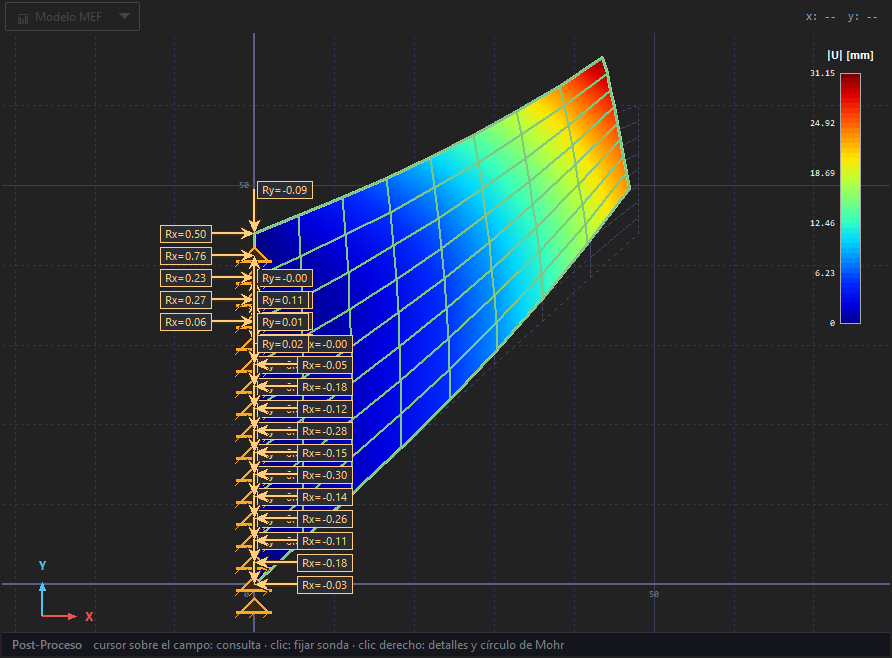
\includegraphics[width=0.78\linewidth]{figuras/fig_cook_deformed}
\caption[Deformada de la membrana de Cook (Q9, $N=8$).]{Post-proceso de EduFEM: configuración deformada de la membrana de Cook (Q9, $N=8$) con el contorno de magnitud de desplazamiento $|U|$. El empotramiento del borde izquierdo y el desplazamiento creciente hacia el extremo libre cargado son visibles sobre la geometría original (en línea punteada).}
\label{fig:cook-def}
\end{figure}


\chapter{Modelo de validación en SAP2000 y solución analítica de Timoshenko}
\label{anexo:sap2000}

Las páginas que siguen son la verificación del caso de la viga realizada con SAP2000, elaborada por el autor, de la que provienen las cifras de contraste que el \autoref{cap:resultados} compara con EduFEM y que el \autoref{anexo:vyv} amplía. El documento reúne la resolución analítica de las tensiones $\sigma_x$, $\sigma_y$ y $\tau_{xy}$ y de los desplazamientos según la teoría de la elasticidad de Timoshenko-Goodier \autocite[art.~21, pp.~39-43]{timoshenko1970elasticity} y el modelado de la misma viga en SAP2000 \autocite[p.~179]{csi2017sap2000} con elementos de cáscara (\emph{shell}). Añade la comparación numérica punto a punto entre ambas referencias en los puntos A, B y C, y el contraste de la deflexión por teoría de vigas, con y sin corrección por cortante. Se incorpora como evidencia documental para dar trazabilidad a esas cifras; sus hojas apaisadas se presentan giradas sobre la hoja vertical, con el folio de la tesis.

Se reproduce tal como fue elaborado, sin rehacer su composición, y por eso conserva convenciones propias, distintas de las del resto del documento. Las principales son cuatro:

\begin{itemize}
    \item escribe «esfuerzo» donde esta tesis escribe «tensión», con el mismo significado;
    \item emplea el punto como separador decimal, frente a la coma del cuerpo y de las tablas del \autoref{anexo:vyv};
    \item expresa las tensiones en kg/cm$^2$, unidad que aquí se escribe kgf/cm$^2$;
    \item usa rótulos y símbolos propios.
\end{itemize}

El peralte $H$, la luz $L$, la base $b$ y la carga distribuida $q$ tienen el significado que les da la Nomenclatura; los demás símbolos del documento no figuran en ella:

\begin{itemize}
    \item $f'_c$, la resistencia característica del hormigón, y $f_y$, el límite de fluencia del acero;
    \item $c = H/2$, el semiperalte, y $l = L/2$, la semiluz;
    \item $I$, el momento de inercia;
    \item $v$, el coeficiente de Poisson, que el cuerpo denota $\nu$.
\end{itemize}

Se conserva además su estilo tipográfico y ortográfico original —títulos en mayúsculas sin tilde, abreviaturas propias y erratas de digitación, como «SAP200», «poison» o «Dezplazamiento»—, junto con las capturas en la resolución en que fueron tomadas.

Dos lecturas del documento requieren una acotación. La primera: la comprobación de que ninguna tensión supera $f'_c = 210$~kgf/cm$^2$ es una lectura de admisibilidad del material, ajena al alcance de este trabajo, que es elástico lineal y no evalúa la capacidad de la sección; otro tanto ocurre con el límite de fluencia del acero de la primera hoja, que no interviene en el análisis. La segunda: en la hoja de discusión de $\sigma_x$, la observación de que en $x = \pm 7$~m «existirá momentos» debe entenderse así: el segundo término de la expresión de Timoshenko-Goodier deja en los apoyos una distribución de $\sigma_x$ autoequilibrada, cuya resultante y cuyo momento son nulos, por lo que el momento flector en los apoyos sigue siendo cero, como corresponde a la viga simplemente apoyada.

% Cada pagina lleva el folio de la tesis (pagecommand={\thispagestyle{fancy}}).
% La pag. 1 del original es vertical (carta, mas ancha que el A4): lleva la misma
% escala que las demas para dejarle margen de encuadernacion. Las 2-11 son
% apaisadas: se giran 90 grados sobre la hoja vertical (angle=90), como una
% figura apaisada, de modo que el numero de pagina queda en su sitio habitual.
% (Con landscape=true pdfpages usa pdflscape y el encabezado no se imprimia.)
% scale y offset dejan libre la franja del encabezado.
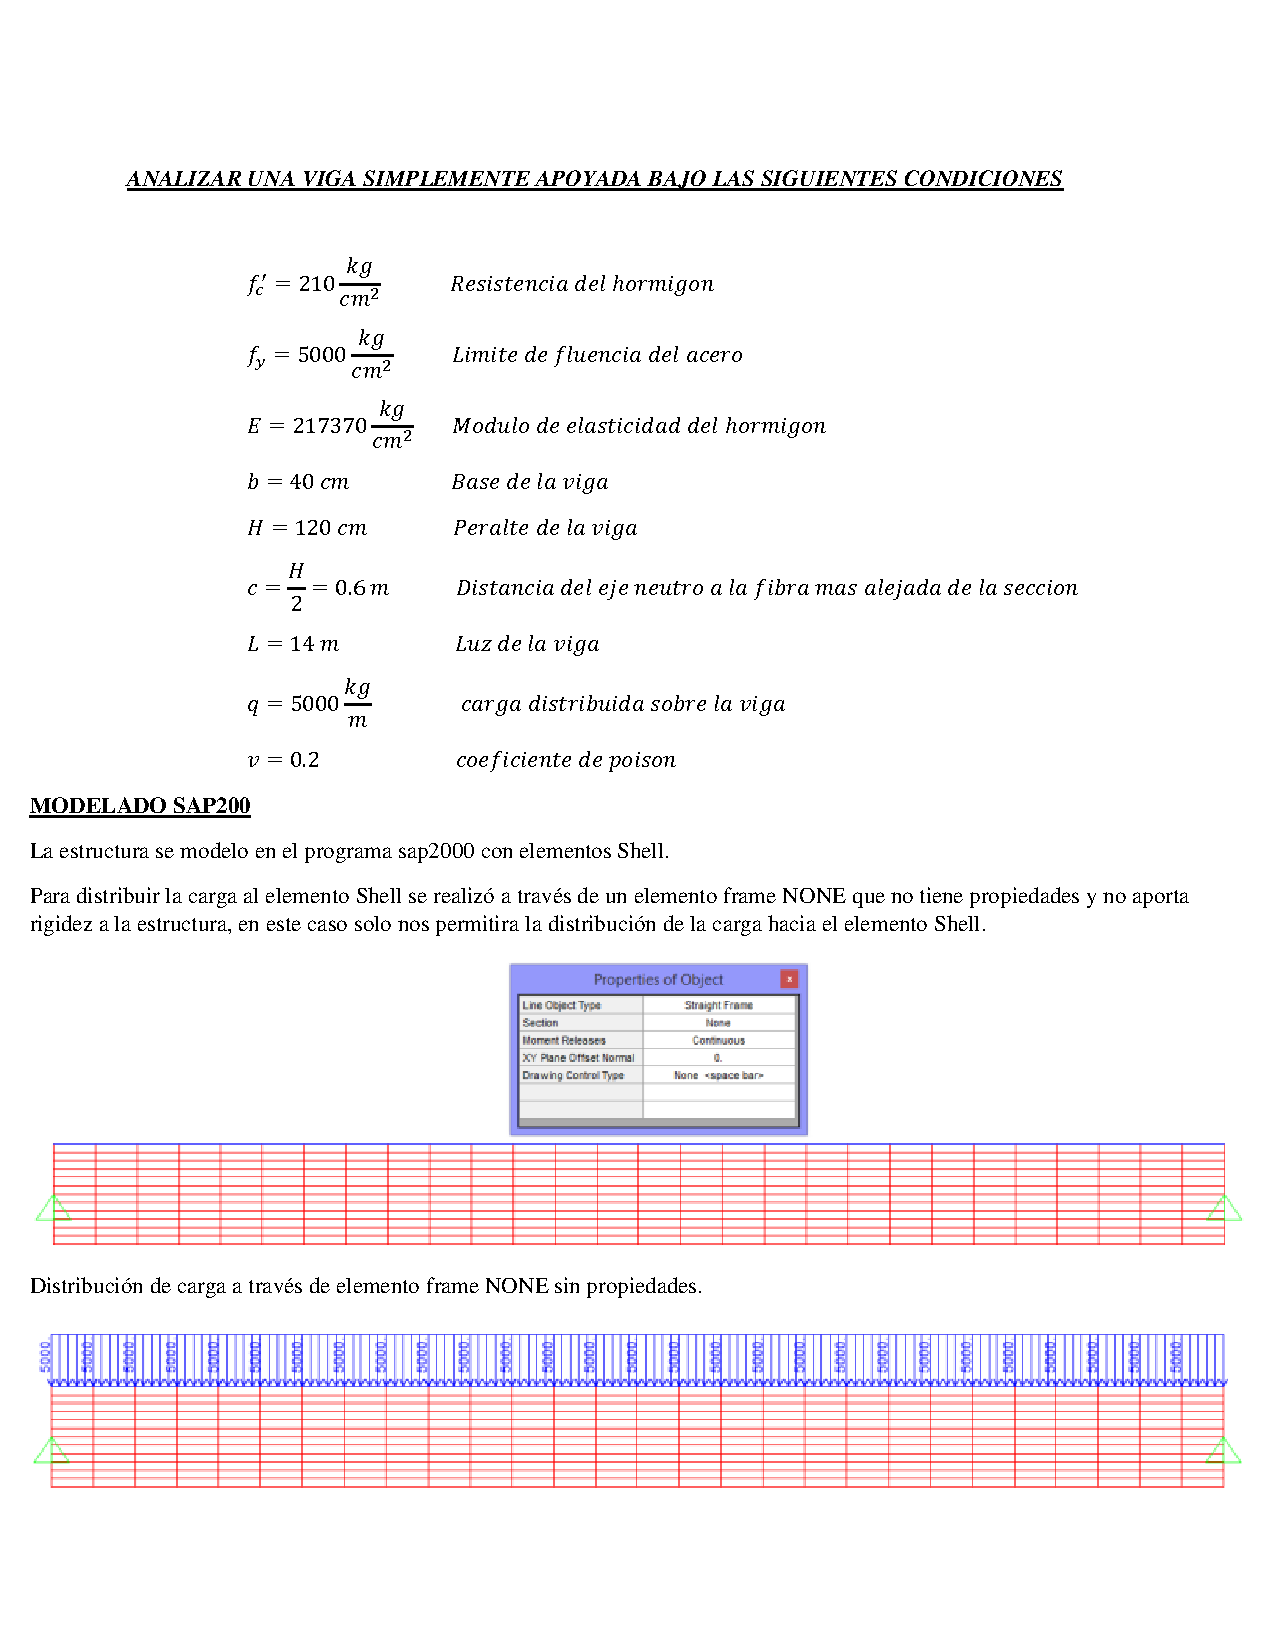
\includepdf[pages=1,scale=0.88,pagecommand={\thispagestyle{fancy}}]{anexos/validacion_sap2000.pdf}
\includepdf[pages=2-11,angle=90,scale=0.88,offset=0 -12pt,pagecommand={\thispagestyle{fancy}}]{anexos/validacion_sap2000.pdf}


\chapter{Formatos de intercambio de datos}
\label{anexo:formatos}

EduFEM intercambia datos con el exterior mediante tres formatos de archivo, cada uno con un propósito distinto: el formato nativo \texttt{.edufem} para guardar y reabrir el proyecto completo sin pérdida de información; un paquete de archivos CSV comprimido para la edición masiva del modelo en una hoja de cálculo; y el formato DXF de dibujo asistido para importar la geometría desde un programa de diseño. Este anexo documenta, como referencia, la estructura de cada uno tal como la lee y escribe el software.

\section{Proyecto nativo (\texttt{.edufem})}

Un archivo \texttt{.edufem} es un documento de texto en formato JSON, codificado en UTF-8, que almacena la totalidad del modelo ---geometría, propiedades, cargas y restricciones--- pero \emph{no} los resultados del cálculo, que EduFEM recomputa al volver a resolver el modelo (tecla F5 o paso al post-proceso). La serialización la produce el método \texttt{to\_dict} de la clase \texttt{ProjectModel}, y la lectura inversa el método \texttt{from\_dict}; ambos comparten el mismo esquema de claves.

El guardado es \textbf{atómico}: el contenido se escribe primero en un archivo temporal del mismo directorio, se fuerza su descarga a disco (\texttt{fsync}) y solo entonces se renombra sobre el destino final mediante \texttt{os.replace}. De este modo, una interrupción a mitad de escritura ---un cierre forzado, un disco lleno o un corte de energía--- nunca deja el archivo original corrupto o truncado: queda intacto el contenido anterior o bien el nuevo completo. La escritura usa una indentación de dos espacios y conserva los caracteres no ASCII (\texttt{ensure\_ascii=False}), de modo que el JSON resultante es legible e inspeccionable con cualquier editor de texto.

El diccionario de nivel superior contiene las claves que detalla la \autoref{tab:edufem-claves}. Las ocho primeras son escalares de configuración global del análisis; las restantes son colecciones de entidades, cada una serializada a su vez con su propio diccionario.

\begin{table}[htbp]
\centering
\caption[Claves del diccionario JSON de un proyecto \texttt{.edufem}.]{Claves del diccionario JSON de nivel superior de un archivo \texttt{.edufem} y significado de cada una. Las ocho primeras son escalares de configuración global del análisis; las seis restantes, colecciones de entidades del modelo.}
\label{tab:edufem-claves}
\begin{tabular}{l p{9.2cm}}
\toprule
\textbf{Clave} & \textbf{Significado} \\
\midrule
\texttt{project\_name}       & Nombre del proyecto (cadena de texto). \\
\texttt{analysis\_type}      & Tipo de análisis: tensión plana o deformación plana. \\
\texttt{element\_type}       & Tipo de elemento de la malla: Q4 o Q9. \\
\texttt{unit\_system}        & Sistema de unidades activo (uno de los ocho predefinidos). \\
\texttt{default\_thickness}  & Espesor por defecto de los elementos. \\
\texttt{gravity\_x}          & Componente $x$ del vector de aceleración de la gravedad. \\
\texttt{gravity\_y}          & Componente $y$ del vector de aceleración de la gravedad. \\
\texttt{include\_gravity}    & Indicador booleano de si la gravedad se incluye como carga. \\
\texttt{nodes}               & Diccionario de nodos indexado por identificador; cada nodo guarda \texttt{id}, \texttt{x}, \texttt{y}. \\
\texttt{elements}            & Diccionario de elementos; cada uno guarda \texttt{id}, \texttt{node\_ids}, \texttt{thickness}, \texttt{material\_name}. \\
\texttt{materials}           & Diccionario de materiales indexado por nombre; cada uno guarda \texttt{name}, \texttt{E}, \texttt{nu}, \texttt{density}. \\
\texttt{nodal\_loads}        & Cargas puntuales por nodo; cada una guarda \texttt{node\_id}, \texttt{fx}, \texttt{fy}. \\
\texttt{surface\_loads}      & Lista de cargas superficiales; cada una guarda \texttt{node\_start}, \texttt{node\_end}, \texttt{q\_start}, \texttt{q\_end}, \texttt{angle}, \texttt{element\_id}. \\
\texttt{boundary\_conditions} & Restricciones por nodo; cada una guarda \texttt{node\_id}, \texttt{restrain\_x}, \texttt{restrain\_y}, \texttt{ux\_value}, \texttt{uy\_value}. \\
\bottomrule
\end{tabular}
\end{table}

La conectividad de cada elemento se almacena en \texttt{node\_ids} como una lista de identificadores: cuatro para un Q4 y nueve para un Q9. Como los identificadores son la identidad pública del nodo (visibles en la interfaz, pueden presentar huecos tras un borrado), el archivo no guarda el mapeo a índices ordinales del sistema lineal: el modelo lo construye bajo demanda a partir de los identificadores ordenados (\autoref{sec:identidad-gdl}), sin depender de que sean contiguos.

\section{Modelo en CSV/Excel (ZIP)}

Para la edición masiva del modelo en una hoja de cálculo, EduFEM exporta e importa sus entidades como un archivo comprimido \texttt{.zip} que contiene un archivo CSV por cada tipo de entidad. El paquete no transporta la configuración del proyecto ni el valor de los desplazamientos prescritos, que solo guarda el formato nativo: al importar, el modelo conserva la configuración del proyecto que lo recibe. Esta vía complementa al formato nativo \texttt{.edufem}: mientras este último es un JSON pensado para guardar y reabrir el proyecto sin edición manual, el paquete de CSV es el formato editable en Excel o LibreOffice.

Cada CSV antepone, en su primera línea, un comentario con las unidades vigentes del proyecto para que el usuario sepa en qué sistema está editando los valores. El comentario se escribe literalmente así, con los rótulos del sistema activo:
\begin{center}\texttt{\# Unidades: longitud=mm, fuerza=N, esfuerzo=MPa}\end{center}
\noindent Nótese que el software emite ahí la palabra \texttt{esfuerzo} como nombre de la tercera unidad; designa lo mismo que este documento llama tensión, y se transcribe tal cual porque es el texto que el usuario encontrará en el archivo. La segunda línea es el encabezado real de columnas y, a partir de la tercera, los datos. Al leer, las líneas que comienzan con \texttt{\#} se descartan. La escritura del ZIP también es atómica, mediante archivo temporal y \texttt{os.replace}, y las celdas de texto que comienzan por un carácter que la hoja de cálculo interpretaría como fórmula (\texttt{=}, \texttt{+}, \texttt{-}, \texttt{@}) se neutralizan anteponiendo un apóstrofo.

La \autoref{tab:csv-archivos} enumera los seis archivos del paquete con sus columnas reales y su contenido.

\begin{table}[htbp]
\centering
\caption[Archivos CSV del paquete de modelo y sus columnas.]{Archivos del paquete CSV comprimido que EduFEM exporta e importa: nombre de cada archivo, columnas reales de su encabezado, en el orden en que se escriben, y entidad que describe.}
\label{tab:csv-archivos}
\begin{tabular}{p{3.6cm} p{5.0cm} p{4.6cm}}
\toprule
\textbf{Archivo} & \textbf{Columnas} & \textbf{Descripción} \\
\midrule
\texttt{nodes.csv} & \texttt{ID}, \texttt{X}, \texttt{Y} & Identificador y coordenadas de cada nodo. \\
\texttt{elements.csv} & \texttt{ID}, \texttt{N1}, \texttt{N2}, \texttt{N3}, \texttt{N4}, \texttt{Espesor}, \texttt{Material} & Identificador, conectividad, espesor y material de cada elemento. \\
\texttt{materials.csv} & \texttt{Nombre}, \texttt{E}, \texttt{nu}, \texttt{densidad} & Nombre, módulo de elasticidad $E$, coeficiente de Poisson $\nu$ y densidad $\rho$. \\
\texttt{nodal\_loads.csv} & \texttt{Nodo}, \texttt{Fx}, \texttt{Fy} & Carga puntual (componentes $F_x$, $F_y$) por nodo. \\
\texttt{boundary\_conditions}\newline\texttt{.csv} & \texttt{Nodo}, \texttt{Restringe\_X}, \texttt{Restringe\_Y} & Restricción por nodo; cada columna de restricción vale \texttt{1} (restringido) o \texttt{0} (libre). \\
\texttt{surface\_loads}\newline\texttt{.csv} & \texttt{Nodo\_Inicio}, \texttt{Nodo\_Final}, \texttt{q\_inicio}, \texttt{q\_final}, \texttt{Angulo} & Carga distribuida sobre la arista entre dos nodos, con magnitudes en cada extremo y ángulo de aplicación. La arista la definen sus dos nodos; el \texttt{element\_id} del JSON es opcional y solo se conserva por compatibilidad con archivos anteriores. \\
\bottomrule
\end{tabular}
\end{table}

Las columnas son fijas, con una salvedad sobre la conectividad de los elementos. La tabla de \texttt{elements.csv} expone \textbf{siempre cuatro columnas de nodo}, \texttt{N1} a \texttt{N4}, que corresponden a los cuatro vértices del cuadrilátero, y el formato editable nunca expone columnas \texttt{N5} a \texttt{N9} ni admite su edición manual. En una malla Q9, los cinco nodos restantes de cada elemento ---los cuatro de arista y el central--- se escriben en \texttt{nodes.csv}, pero no en la conectividad: al importar el paquete en un proyecto configurado como Q9, la expansión automática los vuelve a asociar a cada elemento por sus coordenadas, y en uno configurado como Q4 quedan como nodos sin elemento. Al importar, las cargas y restricciones cuyo nodo no exista en el modelo se descartan silenciosamente, y los materiales se cargan antes que los elementos para que estos puedan referenciarlos por nombre.

\section{Geometría CAD (\texttt{.dxf})}

EduFEM importa la geometría de la malla desde archivos DXF de dibujo asistido, mediante la biblioteca \texttt{ezdxf}. La convención de intercambio es deliberadamente simple: solo se procesan las entidades que residen en la capa denominada \texttt{FEM\_ELEMENTS} (el nombre es configurable, pero ese es el valor por defecto); las demás capas se ignoran por completo. Dentro de esa capa, cada \textbf{polilínea cerrada de exactamente cuatro vértices} se convierte en un elemento cuadrilátero Q4. Una polilínea que no esté cerrada, o que tenga un número de vértices distinto de cuatro, se descarta y se registra una advertencia.

Las coordenadas del DXF se toman literalmente, sin factor de escala; su significado físico (milímetros, metros, pulgadas, etcétera) lo fija el sistema de unidades del proyecto, al estilo de los programas de análisis estructural comerciales. El diálogo de importación permite elegir la unidad de longitud del proyecto antes de importar: si el usuario la cambia, el sistema de unidades del proyecto se actualiza y las coordenadas ya existentes en el modelo se reescalan a la nueva unidad, mientras que los números del DXF se interpretan directamente en ella.

Al construir cada elemento, la importación impone dos reglas de consistencia con el resto del modelo:

\begin{itemize}
  \item \textbf{Orientación antihoraria forzada.} Se calcula el área con signo de la polilínea mediante la fórmula del cordón de zapato (\emph{shoelace}), $A = \tfrac{1}{2}\sum_i (x_i\,y_{i+1} - x_{i+1}\,y_i)$ sobre los vértices recorridos en orden y cerrando el ciclo; si resulta negativa ---orden horario---, se invierte el orden de los vértices. Sin esta corrección, el determinante del Jacobiano sería negativo en todo el elemento, y el comprobador de salud lo advertiría.
  \item \textbf{Compartición automática de nodos.} Los vértices de cada polilínea se deduplican contra los nodos existentes del proyecto dentro de una tolerancia numérica, de modo que dos elementos adyacentes comparten el nodo común en lugar de duplicarlo.
\end{itemize}

La importación es además \textbf{idempotente}: antes de crear un elemento se calcula su firma topológica como el conjunto no ordenado de sus nodos (\texttt{frozenset} de los identificadores) y se compara con las firmas de los elementos ya presentes. Si coincide con uno existente, el elemento se omite y se contabiliza como duplicado. Reimportar el mismo DXF sobre un proyecto ya poblado, por tanto, no genera elementos repetidos.

La función \texttt{import\_dxf} modifica directamente el proyecto que recibe y devuelve un diccionario con el balance de la operación, cuyas claves se describen en la \autoref{tab:dxf-resultado}.

\begin{table}[htbp]
\centering
\caption[Campos del diccionario de resultado de \texttt{import\_dxf}.]{Campos con que la función \texttt{import\_dxf} informa el balance de una importación: nodos y elementos creados, polilíneas omitidas por coincidir con un elemento existente y lista de advertencias. Sirven para comprobar que el archivo se leyó como se esperaba.}
\label{tab:dxf-resultado}
\begin{tabular}{l p{8.4cm}}
\toprule
\textbf{Campo} & \textbf{Significado} \\
\midrule
\texttt{nodes\_added}                & Número de nodos creados (los compartidos por deduplicación no se cuentan). \\
\texttt{elements\_added}             & Número de elementos Q4 efectivamente creados. \\
\texttt{elements\_skipped\_duplicate} & Número de polilíneas omitidas por coincidir su firma topológica con un elemento ya existente. \\
\texttt{warnings}                    & Lista de mensajes de advertencia (polilíneas no cerradas, con número de vértices distinto de cuatro o degeneradas tras la deduplicación). \\
\bottomrule
\end{tabular}
\end{table}

Una malla Q9 no se describe directamente en el DXF, que solo contempla cuadriláteros de cuatro vértices. En un proyecto configurado como Q4, la importación da una malla Q4, convertible después a Q9; en uno configurado como Q9, el diálogo expande cada cuadrilátero importado (nodos de arista y central) y lo informa en el resumen.



